\documentclass{article}
\usepackage{listings}
\usepackage{xcolor}

\title{TCP File Transfer Protocol}
\author{Do Viet Anh BI12-024}

\date{\today}

\lstset{
    language=C,
    basicstyle=\ttfamily,
    keywordstyle=\color{blue}\ttfamily,
    stringstyle=\color{orange}\ttfamily,
    commentstyle=\color{green}\ttfamily,
    morecomment=[l][\color{magenta}]{\#},
    tabsize=4,
    breaklines=true
}

\begin{document}

\maketitle

\date{}

\section{Execute file transfer}

\subsection{Server side}
- Listens for incoming connections on the designated port.\newline 
- Accepts incoming connection requests from clients.\newline 
- Retrieves the filename sent by the client.\newline 
- Receives the file data in segments and saves it into a file on the server.\newline  

\subsection{Client side}
- Establishes connection with Server on specified port.\newline 
- Transmits file name for transfer.\newline 
- Sends file data.\newline 

\section{Protocol design}

\subsection{Server side}

\begin{lstlisting}
    #include <stdio.h>
    #include <stdlib.h>
    #include <string.h>
    #include <arpa/inet.h>
    #define SIZE 1024
    
    void write_file(int sockfd){
        int n;
        FILE *fp;
        char *filename = "2.txt";
        char buffer[SIZE];
    
        fp = fopen(filename, "w");
        if (fp = NULL){
            perror("[-]Error in create file");
            exit(1);
        }
    
        while(1){
            n = recv(sockfd, buffer, SIZE, 0);
            if(n <= 0){
                break;
                return;
            }
            fprintf(fp, "%s", buffer);
            bzero(buffer, SIZE);
        }
        return;
    }
    
    int main(){
      char *ip = "127.0.0.1";
      int port = 8080;
      int e;
    
      int sockfd, new_sock;
      struct sockaddr_in server_addr, new_addr;
      socklen_t addr_size;
      char buffer[SIZE];
    
      sockfd = socket(AF_INET, SOCK_STREAM, 0);
      if(sockfd < 0) {
        perror("[-]Error in socket");
        exit(1);
      }
      printf("[+]Server socket created.\n");
    
      server_addr.sin_family = AF_INET;
      server_addr.sin_port = port;
      server_addr.sin_addr.s_addr = inet_addr(ip);
    
      e = bind(sockfd, (struct sockaddr*)&server_addr, sizeof(server_addr));
      if(e < 0) {
        perror("[-]Error in binding");
        exit(1);
      }
      printf("[+]Biding successfull.\n");
    
      e = listen(sockfd, 10);
      if(e == 0) {
        perror("[-]Listening...\n");
        exit(1);
      }
      else {
        perror("[-]Error in listening");
        exit(1);
      }
      addr_size = sizeof(new_addr);
      new_sock = accept(sockfd, (struct sockaddr*)&new_addr, &addr_size);
      
      write_file(new_sock);
      printf("[+]Data in file.\n");
    
    }
\end{lstlisting}

\subsection{Client side}

\begin{lstlisting}
    #include <stdio.h>
    #include <stdlib.h>
    #include <string.h>
    #include <unistd.h>
    #include <arpa/inet.h>
    #define SIZE 1024
    
    void send_file(FILE *fp, int sockfd){
        char data[SIZE] = {0};
        while(fgets(data, SIZE, fp) != NULL) {
            if (send(sockfd, data, sizeof(data), 0) == -1) {
                perror("[-]Error in sending file.");
                exit(1);
            }
        bzero(data, SIZE);
        }
    }
    
    int main(){
      char *ip = "127.0.0.1";
      int port = 8080;
      int e;
    
      int sockfd;
      struct sockaddr_in server_addr;
      FILE *fp;
      char *filename = "1.txt";
    
      sockfd = socket(AF_INET, SOCK_STREAM, 0);
      if(sockfd < 0) {
        perror("[-]Error in socket");
        exit(1);
      }
      printf("[+]Server socket created.\n");
    
      server_addr.sin_family = AF_INET;
      server_addr.sin_port = port;
      server_addr.sin_addr.s_addr = inet_addr(ip);
    
      e = connect(sockfd, (struct sockaddr*)&server_addr, sizeof(server_addr));
      if(e == -1){  
        perror("[-]Error in connecting");
        exit(1);
      }
      printf("[+]Connected to server.\n");
    
      fp = fopen(filename, "r");
      if (fp = NULL){
        perror("[-]Error in read file");
        exit(1);
      }
    
      send_file(fp, sockfd);
      printf("[+]File data send successfully\n");
      close(sockfd);
      printf("[+]Disconnected from server\n");
    
      return 0;
    }
\end{lstlisting}

\section{Result}

\subsection{Server side}
\begin{figure}[h]
    \centering
    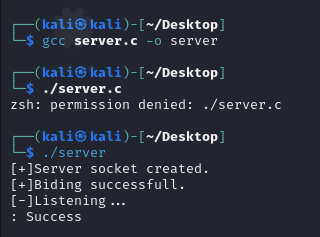
\includegraphics[width=1\textwidth]{server.png}
    \caption{Result of server side}
\end{figure}

\subsection{Client side}
\begin{figure}
    \centering
    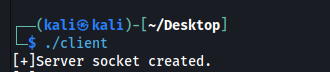
\includegraphics[width=1\textwidth]{client.png}
    \caption{Result of client side}
\end{figure}

\end{document}

